\documentclass[11pt,a4paper]{report}
\usepackage{feram-style}
\graphicspath{{images/}}
\addbibresource{references.bib}

\begin{document}

%% ── Title page ───────────────────────────────────────────────────────────────
\hypersetup{pageanchor=false}
\begin{titlepage}
  \noindent
  
\includegraphics[height=2.2cm]{university_of_prishtina_logo}\hfill
  
\includegraphics[height=2.2cm]{infineon_logo}

  \centering
  \vspace*{0.9cm}
  {\color{ifxblue}\Huge\bfseries HfO$_2$ FeRAM Production System\par}
  \vspace{0.5cm}
  {\LARGE Master Report\par}
  \vspace{1.5cm}
  {\large University of Pristina $\times$ Infineon Collaboration\par}
  \vspace{0.8cm}
  {\large Ontologies Development Workstream\par}
  \vfill
  {\normalsize Project GitHub: \url{https://github.com/OPXHS/Ontologies-Development}\par}
  \vspace{0.4cm}
  {\small\today\par}
\end{titlepage}
\hypersetup{pageanchor=true}
\pagenumbering{roman}

%% ── Abstract ─────────────────────────────────────────────────────────────────
\chapter*{Abstract}
\addcontentsline{toc}{chapter}{Abstract}

%% ── Process ownership ────────────────────────────────────────────────────────
\chapter*{Process Ownership}
\addcontentsline{toc}{chapter}{Process Ownership}
\renewcommand{\arraystretch}{1.35}
\begin{tabularx}{\textwidth}{@{}W{0.72}W{1.02}W{1.26}@{}}
\toprule
\textbf{Student} & \textbf{Assigned chapter} & \textbf{Position in the manufacturing flow} \\
\midrule
Olti Krasniqi & & \\
Art Haxholli & & \\
Fatos Rama & & \\
\bottomrule
\end{tabularx}

\setcounter{tocdepth}{1}
\tableofcontents
\clearpage
\pagenumbering{arabic}

\setstudentheader{Art Haxholli}{ALD HfO$_2$ Process Integration}

\setcounter{chapter}{2}
\chapter{ALD HfO$_2$ Deposition}
\label{chap:ald}

\section{Module Purpose}
\label{sec:ald-module-purpose}

The ALD HfO$_2$ deposition module converts a deposition-ready capacitor region into an electrode-bounded ferroelectric hafnia film whose composition, interfaces, and thermal history are explicit. Within the production-system boundary used here, the module receives the prepared wafer state from the CMOS front end, forms or accepts the bottom-electrode boundary, deposits the HfO$_2$-based layer by an ordered ALD cycle, completes the upper boundary, and applies any route-scoped crystallization treatment. The bottom electrode must precede HZO deposition, but the anneal can occur before or after the upper electrode according to the selected route \cite{kim2020tin,kaatranen2026unif,kashir2021wake,liu2025zrrich}.

Module success is a crystallized film with an orthorhombic ferroelectric contribution inside a functioning capacitor stack, not film deposition alone. ALD provides high-aspect-ratio coverage, yet the deposited material can remain polycrystalline and contain nonferroelectric phases, so geometry and nominal thickness do not establish the required phase state \cite{song2021ferro}. Electrode oxygen exchange, stress, anneal placement, and anneal temperature then determine whether the deposited layer reaches that state or develops monoclinic material, leakage paths, or shorts \cite{silva2023road,kim2020tin,song2023seed,kashir2021wake}. The module hands the resulting capacitor-level material state to downstream integration with its route metadata intact: film composition and thickness, electrode identities and positions, ALD chemistry and sequence, exposure history, and thermal treatment.

\section{Input Condition}
\label{sec:ald-input-condition}

The module assumes a wafer with a defined capacitor region and a surface state ready for the first in-scope preparation or bottom-electrode operation. That input record must preserve substrate or underlying-film identity, prior exposure or vacuum-break history, and any pre-existing interface layer, because a vacuum break is associated with increased carbon and tetragonal-phase stabilization, while deliberately inserted interlayers alter crystallization and defect migration \cite{silva2023road}. Cleaning, seed-layer insertion, and bottom-electrode formation are therefore module operations unless a route explicitly records them as already complete.

The ledger does not define one complete incoming wafer state. Its seven input-condition claims come from three sources and mainly specify the intended HZO film---10 or 25~nm, nominal 1:1 Hf:Zr, and one 50--200~$\mu$m capacitor-diameter range---rather than the underlying CMOS surface \cite{kim2020tin,zhang2015inductive}. A TiN/HZO/TiN route records a 10~nm Hf$_{0.5}$Zr$_{0.5}$O$_2$ target \cite{tsai2022stress}. The remaining eleven sources provide no claim under the input-condition target, so substrate material and incoming topography cannot be completed by inference.

\section{The Shape of the Evidence}
\label{sec:ald-evidence-shape}

The literature reports routes, not recipes. A reported temperature, duration, pressure, or cycle count becomes interpretable only with the configuration that produced it: precursor and oxidant chemistry, reactor mode, film composition and thickness, electrode identities and positions, exposure history, anneal placement, and measurement protocol. The chapter therefore reports two evidence objects. A \emph{literature window} is the conditioned span documented by several routes; a \emph{route instance} is one value inside, at the edge of, or beyond that span. Neither object is a recommendation, and an instance never becomes a norm merely because it is precise.

The useful synthesis is directional coupling between variables. Electrode boundary condition determines anneal placement: an uncapped route anneals before the upper electrode, whereas a capped route anneals after it \cite{song2021ferro,zhang2015inductive}. Deposition temperature increases oxygen-vacancy indicators and dead-layer formation; the higher vacancy state then raises remanent polarization while bringing fatigue onset to a lower cycle count \cite{choi2022chamber}. Precursor-purge duration changes retained carbon and nitrogen impurities and also shifts breakdown: reduced purge does not completely remove ligands, but extending the studied purge from 3 to 90~s changes the same capacitor series from no fatigue or breakdown through $10^9$ cycles to breakdown at $6\times10^7$ cycles \cite{choi2025purge}. These observations establish directed dependencies without claiming that the intermediate impurity signal alone explains the breakdown direction.

Transfer between routes would require demonstrated equivalence of every variable that changes the relevant outcome. For a deposition value, that includes precursor identity and delivery mode, line and source temperatures, co-reactant exposure, reactor mode, substrate temperature, cycle architecture, composition, and thickness. For a thermal value, it additionally includes the electrode material, whether the film is capped, anneal position, ambient, ramp, duration, and preceding exposure. For an electrical result, stack area, conditioning state, waveform, field or voltage, frequency, and driven electrode must match. When those conditions are absent, the value remains route-scoped; when a condition is unreported, the gap remains an assertion rather than an invitation to infer it.

\subsection{Invariant and Route-Variable Sequence}
\label{sec:ald-sequence-invariance}

Bottom-electrode formation precedes HZO deposition in every route that states this relation. The invariant appears for sputtered TiN and W bottom electrodes and for wafer-scale SS/SL, Zr-rich, and W/HZO/W stacks \cite{kim2020tin,kaatranen2026unif,liu2025zrrich,kashir2021wake}. No ledger claim reverses the relation. This supports a necessary \texttt{precedes} assertion in the later ontology rather than a preferred process order.

Anneal placement is route-variable because the electrode boundary at heating changes from one configuration to another. PDA is recorded as uncapped RTA and PMA as RTA after TiN capping; other routes place post-deposition annealing before the upper electrode or post-metallization annealing after it \cite{song2021ferro,choi2022chamber,song2023seed}. One study deliberately compares both orders, applying RTP before top-electrode deposition to its uncapped sample and after top-electrode deposition to its capped sample \cite{zhang2015inductive}. A wafer-scale route narrows placement further to after top-TiN patterning but before bottom-TiN localization \cite{kaatranen2026unif}. These are route-scoped \texttt{precedes} relations; none can replace the bottom-electrode invariant.

\subsection{First-Order and Second-Order Variables}
\label{sec:ald-variable-order}

First-order variables are those for which the ledger records a qualitative change of phase state or device survival. Anneal temperature and its placement relative to capping are first-order: top-electrode temperature and capped versus uncapped order change monoclinic or orthorhombic phase outcomes, while annealing W/HZO/W above 720~$^\circ$C produces large leakage and shorts \cite{kim2020tin,zhang2015inductive,kashir2021wake}. Deposition temperature is first-order because it changes whether an interfacial dead layer forms and shifts the vacancy-mediated polarization--fatigue state \cite{choi2022chamber}. Precursor-purge duration is first-order because the studied series crosses from survival beyond $10^9$ cycles to dielectric breakdown, not merely between two numerical values \cite{choi2025purge}. Electrode material and oxygen affinity are first-order because oxygen-gettering TiN promotes the ferroelectric phase, while oxygen-supplying RuO$_2$/IrO$_2$ and oxidation-resistant alternatives change the reported endurance boundary \cite{silva2023road,liao2023postmoore,kim2020tin}. Oxidant exposure is also first-order in the supported W/HZO/W route: short ozone pulses produce pinched loops, whereas a 15~s pulse produces an open loop \cite{kashir2021wake}.

Second-order variables shift a value inside a demonstrated working configuration without a ledger-supported qualitative transition. The precursor-source temperatures, ALD chamber pressure, sputter power, and exact cycle or supercycle count are second-order on the present evidence: the ledger records settings or numerical trends, but no isolated phase change or device-destruction threshold for those variables \cite{choi2022chamber,choi2025purge,kashir2021wake}. Electrode-deposition pressure is a position-specific exception rather than evidence that every pressure is first-order, because TiN top-electrode microtexture is reported to decide the resulting crystalline phase \cite{silva2023road}. Gas-flow rates, anneal ambient independent of temperature and placement, and precursor delivery-mode effects remain unclassified because the ledger does not isolate their qualitative impact.

Evidence density and importance are independent. The first-purge target contains only three claims from one source, yet its purge-duration series produces one of the ledger's largest outcome changes: endurance falls from beyond $10^9$ to $6\times10^7$ cycles as the precursor purge extends from 3 to 90~s \cite{choi2025purge}. Sparse coverage therefore reduces confidence in transfer, not the observed effect within that route.

\section{Pre-Deposition Preparation}
\label{sec:ald-pre-deposition}
\subsection{Starting Film, Substrate, and Device Conditions}
\label{sec:ald-starting-film}

The starting-film specification constrains the cycle architecture that follows. A 10~nm, nominally equimolar HZO condition is paired with a $250\,^{\circ}$C wafer temperature and 50--200~$\mu$m capacitor diameters in one TiN route, whereas another route records a 25~nm HZO film without supplying the same device dimensions \cite{kim2020tin,zhang2015inductive}. A TiN/HZO/TiN route records a 10~nm Hf$_{0.5}$Zr$_{0.5}$O$_2$ target \cite{tsai2022stress}. The input-condition target contains seven claims from three of fourteen sources; it leaves substrate material, incoming topography, and prior thermal state unreported for the other eleven.
\subsection{Surface Cleaning and Exposure Control}
\label{sec:ald-surface-cleaning}

Surface cleaning establishes the chemical state on which the first in-scope interface or electrode is formed. Its process function is to remove residual contamination and to make exposure history explicit; the failure mode documented in the ledger is that a pre-deposition vacuum break increases carbon and stabilizes the tetragonal phase \cite{silva2023road}. The operation therefore controls a boundary condition for crystallization rather than merely improving visual cleanliness.

The available cleans are purpose- and position-specific. One substrate route applies SPM followed by RCA SC-1/SC-2, while another uses sequential ultrasonic acetone, ethanol, and DI-water cleaning \cite{choi2022chamber,song2023seed}. Wet chemistry used after electrode formation serves a different operation and is not evidence for the incoming preclean \cite{choi2025purge,kim2020tin,neuber2022peald}. Six of fourteen sources contribute surface-preclean claims; the remaining eight do not report the preclean chemistry or exposure control.
\subsection{Interface and Seed-Layer Engineering}
\label{sec:ald-interface-seed}

Interface layers direct crystallization and defect transport. ZrO$_2$, Al$_2$O$_3$, TiO$_2$, and LSMO interlayers are reported below ferroelectric hafnia to alter crystallization, while Al$_2$O$_3$ barriers restrict defect migration or grain-boundary conduction \cite{silva2023road,liao2023postmoore}. The same Al$_2$O$_3$ insertion introduces voltage division and a depolarization field, so the barrier function and electrical penalty are coupled rather than independently selectable \cite{silva2023road,liao2023postmoore}.

Interface position determines which mechanism is available. Top, bottom, dual, and unseeded ZrO$_2$ configurations remain separate specimens; the dual layers are resolved at both HZO interfaces, and their phase and cycling response cannot be assigned to a generic ``seeded'' class \cite{song2023seed}. Pt insertion suppresses the W/HZO interfacial layer and raises the interface barrier, whereas a Zr-rich middle layer divides HZO into a trilayer architecture \cite{kashir2021wake,liu2025zrrich}. In Si-doped stacks, a thicker PEALD SiO$_2$ monolayer shifts the doping concentration relative to thermal ALD, so nominal cycle ratios do not assert equal composition \cite{neuber2022peald}. Nine sources cover interface preparation; none supplies a cross-route equivalence test for these alternatives.

\section{Electrode Integration}
\label{sec:ald-electrode-integration}
\subsection{Bottom Electrode Formation}
\label{sec:ald-bottom-electrode}

Bottom-electrode formation fixes the mechanical and oxygen-exchange boundary before HZO growth. Supported routes sputter TiN, W, or a TiN/Ru stack before oxide deposition; the SNAP route instead forms TiN and HZO sequentially in one ALD chamber without a vacuum break \cite{silva2023road,choi2022chamber,zhang2015inductive,kaatranen2026unif}. The position is invariant even though material, method, and thickness vary.

A TiN/HZO/TiN route records a 15~nm bottom TiN layer sputtered at 100~W, 2.5~mTorr, with Ar and N$_2$ flows of 50 and 3~sccm \cite{tsai2022stress}. The thickness lies inside the ledger's 10--90~nm electrode envelope, the power lies between the reported 50 and 250~W instances, the pressure extends the sputter-pressure low end below 5.0~mTorr, and the gas-flow quantities have no prior sccm entry. These relations locate one route against the evidence window without transferring its settings.

\subsection{Top Electrode and Capping}
\label{sec:ald-top-electrode}

Top-electrode and capping formation determine the boundary condition present during subsequent heating. Some routes deposit a TiN, Ni, or W top electrode before crystallization, while the seed-layer PDA route anneals before its upper TiN is added \cite{choi2022chamber,song2023seed,zhang2015inductive,kashir2021wake}. In the purge study, the W capping layer and the later Pt characterization contact are separate operations; Au/Pd hard masks and Ti/Au contacts likewise do not become capacitor electrodes merely because they are metallic \cite{choi2025purge,kim2020tin,kaatranen2026unif}.

A TiN/HZO/TiN route records a 15~nm sputtered TiN top electrode but no separate top-electrode power, gas flow, or pressure \cite{tsai2022stress}. Its thickness is inside the 10--90~nm literature envelope, but the missing deposition conditions prevent the bottom-electrode settings from being copied to the top position.

\subsection{Electrode Material Selection and Interface Consequences}
\label{sec:ald-electrode-material-selection}

Electrode oxygen affinity directs the film's phase and defect boundary. TiN gettering and bottom-electrode oxidation promote the ferroelectric phase, while RuO$_2$ and IrO$_2$ supply oxygen and are associated with improved endurance relative to oxygen-gettering alternatives \cite{silva2023road,kim2020tin}. W contributes a tensile-strain route through its low thermal-expansion behavior, and a W/Pt/HZO/W stack deliberately assigns top W and bottom Pt to combine mechanical stress with a sharper oxide interface \cite{silva2023road,kashir2021wake}.

Electrode position also changes the mechanism for the same nominal material. TiN top-electrode microtexture depends on deposition pressure, and room-temperature TiN suppresses monoclinic formation through stress-induced crystallization, whereas deposition at $500\,^{\circ}$C produces a confirmed monoclinic phase \cite{silva2023road,kim2020tin}. Material identity, stack position, deposition condition, and anneal placement must therefore remain separate properties in the route record.

\Needspace*{9\baselineskip}
\begingroup\feramtablesetup
\begin{longtable}{@{}P{2.61cm}P{1.76cm}P{2.40cm}P{1.62cm}P{2.75cm}P{3.45cm}@{}}
\caption{Electrode integration routes and stack conditions}\label{tab:ald-electrode-integration}\\
\toprule
\textbf{Stack position} & \textbf{Electrode} & \textbf{Integration method} & \textbf{Thickness} & \textbf{Process condition} & \textbf{Source\slash configuration} \\
\midrule
\endfirsthead
\caption[]{Electrode integration routes and stack conditions \textnormal{\itshape(continued)}}\\
\toprule
\textbf{Stack position} & \textbf{Electrode} & \textbf{Integration method} & \textbf{Thickness} & \textbf{Process condition} & \textbf{Source\slash configuration} \\
\midrule
\endhead
\midrule
\multicolumn{6}{r@{}}{\contnote}\\
\endfoot
\bottomrule
\endlastfoot
Three-dimensional capacitor & \nc & Conformal ALD & 10 nm & High-aspect 1T--1C FeRAM & Song configuration \cite{song2021ferro} \\
Bottom and top & TiN & In-tool SNAP ALD & \nc & Without vacuum break & Roadmap configuration \cite{silva2023road} \\
Bottom and top & TiN & DC sputtering & 50 nm & Reference capacitor & Choi configuration \cite{choi2022chamber} \\
Bottom & W & DC magnetron sputtering & \nc & 3.3 W\slash cm$^2$; 5.0 mTorr Ar & W baseline \cite{choi2025purge} \\
Top capping & W & DC magnetron sputtering & 20 nm & Reduced deposition time & W capping configuration \cite{choi2025purge} \\
Top contact & Pt & Shadow-mask deposition & 50 nm & Electrical characterization & Pt contact configuration \cite{choi2025purge} \\
Bottom and top & TiN & RF sputtering & 90 nm & 250 W; Ar:N$_2$ 20:1; RT or 500$^\circ$C & TiN temperature study \cite{kim2020tin} \\
Hard mask & Au\slash Pd & Sequential e-beam evaporation & 85\slash 3 nm & Sequential deposition & Hard-mask configuration \cite{kim2020tin} \\
Upper & TiN & RF sputtering & 50 nm & 400 $\mu$m; 29 ohm\slash sq & Seed-layer device \cite{song2023seed} \\
Bottom stack & TiN\slash Ru & \nc & 20\slash 100 nm & 300 nm SiO$_2$ base & Induced-crystallization capacitor \cite{zhang2015inductive} \\
Top & Ni & Sputtering & 50 nm & 50 W cluster system & Ni-top capacitor \cite{zhang2015inductive} \\
Bottom and top & TiN & Bottom ALD; top PVD & 10 nm & Silicon-doped hafnia capacitor & Neuber configuration \cite{neuber2022peald} \\
Bottom and top & TiN & Reactive sputtering & 30 nm & Superlattice capacitor & Wafer-scale configuration \cite{kaatranen2026unif} \\
Electrical contacts & Ti\slash Au & Evaporation and lift-off & \nc & Contacts to TiN electrodes & Wafer-scale configuration \cite{kaatranen2026unif} \\
Bottom and top & W & Magnetron sputtering & 30 nm & Room temperature; top 80$\times$80 $\mu$m$^2$ & Zirconium-rich capacitor \cite{liu2025zrrich} \\
Bottom and top & W & Bottom sputter; top RF sputter & 50 nm & Room temperature; 30$\times$30--100$\times$100 $\mu$m$^2$ & Wake-up-free capacitor \cite{kashir2021wake} \\
Hybrid interfaces & Top W; bottom Pt & RTA-integrated stack & \nc & Mechanical stress with Pt interface & Hybrid capacitor \cite{kashir2021wake} \\
Gate stack & Polysilicon\slash TiN & \nc & \nc & 28 nm CMOS FeFET stack & FeFET configuration \cite{mikolajick2018mrs} \\
\end{longtable}
\endgroup

\section{ALD Film Formation}
\label{sec:ald-film-formation}
\subsection{Metal-Precursor Dose}
\label{sec:ald-metal-dose}

Precursor identity determines the delivery conditions that can be interpreted together. The ledger spans cyclopentadienyl, alkylamide, TEMA-, and TDMA-based precursors; organometallic ligands are associated with residual impurities, and the alkylamide family carries a reported thermal-stability limit \cite{song2021ferro,silva2023road}. In the most resolved TEMA-based PEALD route, bubbler temperatures, hotter downstream manifolds, Ar-assisted dosing at 80~mTorr, and unequal Hf and Zr pulse lengths form one delivery system \cite{choi2025purge}. Separating any one number from that system removes the condensation-control and dose context.

One TiN/HZO/TiN route records TEMAH at 90~$^\circ$C and TEMAZ at 110~$^\circ$C for deposition at 250~$^\circ$C \cite{tsai2022stress}. The TEMAH temperature matches a prior 90~$^\circ$C instance, but the TEMAZ temperature exceeds the previously documented 85 and 90~$^\circ$C values \cite{choi2025purge,kashir2021wake}. This is an extension, not a contradiction: the route omits delivery mode and line temperature, which are the conditions required to reconcile absolute source temperatures.
\subsection{First Purge}
\label{sec:ald-first-purge}

The first purge is the cycle boundary that separates the metal-precursor dose from co-reactant admission. In the process model, its function is to clear the reaction space before the oxidant arrives; incomplete clearing is represented by retained precursor ligands, and the measured reduced-purge films retain carbon and nitrogen impurities \cite{choi2025purge}. This definition supplies the operation's role without turning one experimental duration into a default.

Purge duration controls both retained chemistry and device survival in the only resolved series. Ar at 80~mTorr is held as the purge environment while duration spans 3--90~s; the 3~s device shows no fatigue or breakdown through $10^9$ cycles, but the 90~s device breaks at $6\times10^7$ cycles \cite{choi2025purge}. Only one of fourteen sources reports the first purge as its own target, leaving thirteen without a first-purge duration or independent failure comparison.

\subsection{Co-Reactant Dose}
\label{sec:ald-co-reactant-dose}

Co-reactant exposure determines how each adsorbed precursor half-cycle is oxidized. Thermal routes report H$_2$O or O$_3$, while plasma-enhanced routes report oxygen-plasma exposures; one PEALD sequence assigns different power--duration pairs to the Hf and Zr subcycles \cite{song2021ferro,choi2025purge,kim2020tin,song2023seed}. In W/HZO/W, increasing the ozone pulse from below 5~s to 15~s changes the pristine response from pinched to open hysteresis and reduces carbon at the high-dose condition \cite{kashir2021wake}. Oxidant identity and exposure must therefore remain attached to the metal subcycle and electrode stack.

The TiN/HZO/TiN route does not report its oxidant \cite{tsai2022stress}. It is not evidence that the route used no oxidant, nor may H$_2$O be supplied by analogy. The recorded gap shows that an otherwise ordered route can leave a first-order cycle variable unspecified.

\subsection{Second Purge}
\label{sec:ald-second-purge}

The second purge is the cycle boundary between the co-reactant exposure and the next metal-precursor dose. In the process model, it restores a separated starting state for repetition; failure to clear the preceding exposure would leave the next dose without the temporal isolation that defines the recorded ALD sequence. This is a functional operation definition, not a reported duration.

The evidence base identifies only nitrogen as the purge and carrier gas in one thermal HZO route \cite{zhang2015inductive}. One of fourteen sources therefore covers the second-purge target, while thirteen report no second-purge gas; all fourteen omit a second-purge duration, pressure, and measured failure mode. The chapter preserves that evidence gap rather than copying first-purge conditions into the second purge.

\subsection{Cycle and Supercycle Architecture}
\label{sec:ald-cycle-architecture}

Supercycle count is a dependent variable in the thermal HZO temperature series. Holding film thickness at 10~nm, the route uses 56, 61, and 68 supercycles as chamber temperature rises from 120 to 250~$^\circ$C because growth per supercycle decreases with temperature \cite{choi2022chamber}. The count encodes the deposition condition rather than specifying it independently.

Cycle architecture can change composition sequence while total count or thickness remains fixed. A nanolaminate series holds 120 combined HfO$_2$/ZrO$_2$ cycles while changing block length, the SS/SL comparison reaches 5.5~nm through alternating single cycles or grouped symmetric blocks, and discrete-feeding ALD repeats the precursor half-cycle before the reactant half-cycle \cite{silva2023road,song2023seed,kaatranen2026unif}. A separate PEALD route uses a 3:2 Hf:Zr dose cycle to target nominal Hf$_{0.5}$Zr$_{0.5}$O$_{2-x}$ \cite{choi2025purge}.

A TiN/HZO/TiN route records a 1:1 HfO$_2$:ZrO$_2$ cycle ratio for nominal Hf$_{0.5}$Zr$_{0.5}$O$_2$ \cite{tsai2022stress}. Its ratio sits inside the documented architectures and matches one W/HZO/W route approximately, yet the 3:2 PEALD example proves that nominal equimolar composition does not entail 1:1 cycling \cite{choi2025purge,kashir2021wake}.

\Needspace*{9\baselineskip}
\begingroup\feramtablesetup
\begin{longtable}{@{}P{2.16cm}P{2.55cm}P{1.91cm}P{3.03cm}P{1.80cm}P{3.13cm}@{}}
\caption{Documented ALD cycle chemistries and operating windows}\label{tab:ald-cycle-windows}\\
\toprule
\textbf{Film\slash stack} & \textbf{Hf precursor} & \textbf{Co-reactant} & \textbf{Cycle\slash timing} & \textbf{T\slash P window} & \textbf{Source\slash condition} \\
\midrule
\endfirsthead
\caption[]{Documented ALD cycle chemistries and operating windows \textnormal{\itshape(continued)}}\\
\toprule
\textbf{Film\slash stack} & \textbf{Hf precursor} & \textbf{Co-reactant} & \textbf{Cycle\slash timing} & \textbf{T\slash P window} & \textbf{Source\slash condition} \\
\midrule
\endhead
\midrule
\multicolumn{6}{r@{}}{\contnote}\\
\endfoot
\bottomrule
\endlastfoot
HfO$_2$ & Cp$_2$HfMe$_2$; (MeCp)$_2$HfMe$_2$; (MeCp)$_2$Hf(OMe)Me; Hf(NEtMe)$_4$; Hf(NMe$_2$)$_4$ & H$_2$O, O$_2$ plasma, O$_3$ & \nc & 250--300 $^\circ$C stability & Precursor and oxidant survey \cite{song2021ferro} \\
HfO$_2$\slash ZrO$_2$ & TEMAHf & H$_2$O, O$_3$, O$_2$ plasma, H$_2$O$_2$ & DF-ALD repeats precursor half-cycle & \nc & DF-ALD review \cite{silva2023road} \\
TiN\slash 10 nm Hf$_{0.5}$Zr$_{0.5}$O$_2$\slash TiN & \nc & H$_2$O & 56--68 supercycles & 120--250 $^\circ$C & Thermal ALD chamber study \cite{choi2022chamber} \\
10 nm Hf$_{0.5}$Zr$_{0.5}$O$_2$ & TEMA-Hf & O$_2$ plasma, 3--6 s & 1.0\slash 1.5 s doses; 3--90 s Ar purge & 260 $^\circ$C; 80 mTorr & 3:2, 17-supercycle PEALD study \cite{choi2025purge} \\
Hf$_{0.5}$Zr$_{0.5}$O$_2$ & TDMA-Hf & O$_3$, 400 g m$^{-3}$ & \nc & \nc & High-concentration O$_3$ ALD \cite{kim2020tin} \\
Hf$_{0.5}$Zr$_{0.5}$O$_2$ nanolaminate & TEMA-Hf & O$_2$ plasma, 200 W & $(5,5)\times12$--$(60,60)\times1$; 120 cycles & 250 $^\circ$C & Seed-layer PEALD study \cite{song2023seed} \\
Hf$_{0.5}$Zr$_{0.5}$O$_2$ & \nc & H$_2$O & N$_2$ second purge & 200 $^\circ$C & Thermal ALD study \cite{zhang2015inductive} \\
10 nm HfO$_2$\slash SiO$_2$ & HfCl$_4$ & H$_2$O & 10:1--27:1 HfO$_2$:SiO$_2$ cycles & 300 $^\circ$C & Thermal HSO process \cite{neuber2022peald} \\
Hybrid HfO$_2$\slash SiO$_2$ & \nc & O$_2$, Ar plasma & 1 SiO$_2$:16--32 HfO$_2$ cycles & 50 $^\circ$C SiO$_2$ PEALD & Hybrid HSO process \cite{neuber2022peald} \\
5.5 nm SS-\slash SL-Hf$_{0.5}$Zr$_{0.5}$O$_2$ & TDMAHf & H$_2$O & SS $(1+1)\times27$; SL $5(5+6)+5$ & 200 $^\circ$C & Thermal superlattice ALD \cite{kaatranen2026unif} \\
Hf$_{0.5}$Zr$_{0.5}$O$_2$\slash ZrO$_2$\slash Hf$_{0.5}$Zr$_{0.5}$O$_2$ & TEMAH & Oxygen plasma & \nc & 250 $^\circ$C & Zr-rich stack PEALD \cite{liu2025zrrich} \\
10 nm Hf$_{0.5}$Zr$_{0.5}$O$_2$ on W & \nc & O$_3$, 276 g Nm$^{-3}$ & 1:1 Hf:Zr; 2--15 s O$_3$ pulse & 250 $^\circ$C; 90 $^\circ$C precursors & O$_3$-pulse ALD study \cite{kashir2021wake} \\
\end{longtable}
\endgroup

\begin{figure}[htbp]
  \centering
  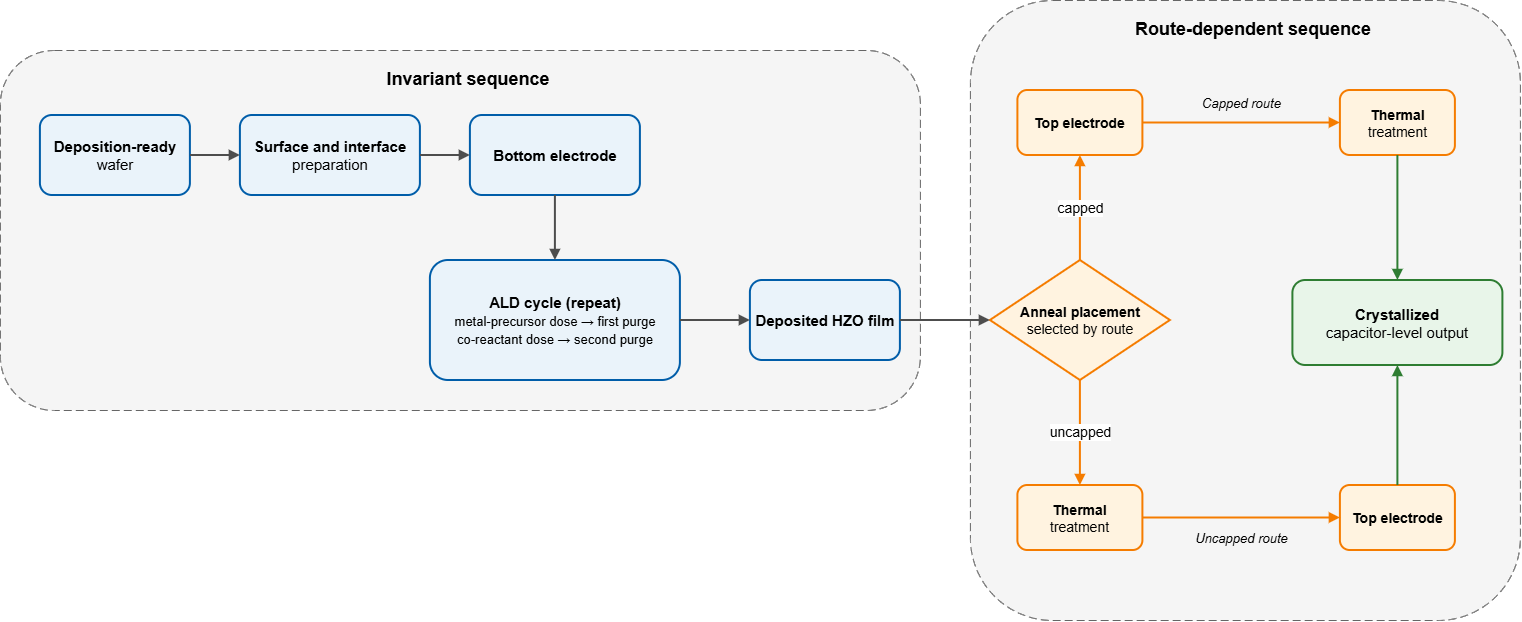
\includegraphics[
    width=0.95\textwidth,
    keepaspectratio
  ]{images/figure3_1_ald_hfo2_module_process_flow.png}
  \caption{ALD HfO$_2$ module process flow}
  \label{fig:ald-flow}
\end{figure}

\section{Post-Deposition Thermal Treatment}
\label{sec:ald-post-deposition-thermal}

Thermal treatment converts the deposited film toward the route's crystalline state and can also terminate the usable process window. A $650\,^{\circ}$C seed-layer anneal increases monoclinic phase and degrades ferroelectric behavior, while W/HZO/W annealing above $720\,^{\circ}$C causes large leakage and short circuits \cite{song2023seed,kashir2021wake}. Temperature, time, ambient, and electrode boundary must therefore be evaluated as one treatment event.

Electrode state determines where the treatment is placed. PDA is recorded without a TiN cap or before the upper electrode, PMA follows capping or the top electrode, and a deliberate capped--uncapped comparison applies RTP on opposite sides of top-electrode deposition \cite{song2021ferro,choi2022chamber,song2023seed,zhang2015inductive}. A wafer-scale route anneals after top-TiN patterning but before bottom-TiN localization, while another pre-anneals the bottom TiN before HZO specifically to isolate top-electrode stress \cite{kaatranen2026unif,kim2020tin}. The sub-$400\,^{\circ}$C BEOL-compatible route is a module limitation; higher-temperature examples do not override its stated budget \cite{silva2023road,neuber2022peald}.

The TiN/HZO/TiN route records RTP at $500\,^{\circ}$C for 30~s in N$_2$ \cite{tsai2022stress}. The complete temperature--time--ambient tuple exactly matches a TiN/HZO/TiN post-metallization condition reported by Choi et al. \cite{choi2022chamber}. This is the strongest cross-route corroboration because stack, temperature, duration, and ambient agree without averaging. Thirteen sources cover thermal treatment, but only one reports a heating ramp; ramp profile remains the section-level evidence gap.

\Needspace*{9\baselineskip}
\begingroup\feramtablesetup
\begin{longtable}{@{}P{2.31cm}P{2.79cm}P{2.06cm}P{1.70cm}P{2.22cm}P{3.50cm}@{}}
\caption{Reported post-deposition treatment conditions}\label{tab:ald-post-deposition}\\
\toprule
\textbf{Film\slash stack} & \textbf{Anneal sequence} & \textbf{Temperature} & \textbf{Time} & \textbf{Ambient} & \textbf{Source\slash condition} \\
\midrule
\endfirsthead
\caption[]{Reported post-deposition treatment conditions \textnormal{\itshape(continued)}}\\
\toprule
\textbf{Film\slash stack} & \textbf{Anneal sequence} & \textbf{Temperature} & \textbf{Time} & \textbf{Ambient} & \textbf{Source\slash condition} \\
\midrule
\endhead
\midrule
\multicolumn{6}{r@{}}{\contnote}\\
\endfoot
\bottomrule
\endlastfoot
HfO$_2$ & PDA; uncapped RTA & \nc & \nc & \nc & PDA definition \cite{song2021ferro} \\
HfO$_2$ & PMA after TiN capping & \nc & \nc & \nc & PMA definition \cite{song2021ferro} \\
HfO$_2$--ZrO$_2$ & Low-temperature crystallization & $<400\,^{\circ}\mathrm{C}$ & \nc & \nc & BEOL compatibility \cite{silva2023road} \\
Hf$_{0.5}$Zr$_{0.5}$O$_2$ & PMA by RTA & $400$--$700\,^{\circ}$C & 30~s & N$_2$ & Temperature series \cite{choi2022chamber} \\
Hf$_{0.5}$Zr$_{0.5}$O$_2$ & RTA; $50\,^{\circ}$C\slash s ramp & $600\,^{\circ}$C & 30~s & N$_2$, 1~atm & PEALD capacitor stack \cite{choi2025purge} \\
TiN\slash Hf$_{0.5}$Zr$_{0.5}$O$_2$\slash TiN & PMA by RTA & $400\,^{\circ}$C & 60~s & N$_2$ & Top-electrode anneal \cite{kim2020tin} \\
TiN\slash Hf$_{0.5}$Zr$_{0.5}$O$_2$\slash TiN & Forming-gas furnace anneal & $400\,^{\circ}$C & 30~min & 5\% H$_2$ + 95\% N$_2$ & Hydrogen treatment \cite{kim2020tin} \\
Hf$_{0.5}$Zr$_{0.5}$O$_2$ & PDA before upper electrode & $450$--$650\,^{\circ}$C & 30~s & N$_2$ & Seed-layer study \cite{song2023seed} \\
Ni-capped Hf$_{0.5}$Zr$_{0.5}$O$_2$ MIM & RTP after top-electrode deposition & 823~K & 30~s & N$_2$ & Capped structure \cite{zhang2015inductive} \\
Uncapped Hf$_{0.5}$Zr$_{0.5}$O$_2$ MIM & RTP before top-electrode deposition & \nc & \nc & \nc & Uncapped comparison \cite{zhang2015inductive} \\
Si:HfO$_2$ & Anneal after stack formation & $800\,^{\circ}$C & 20~s & N$_2$ & Polar-phase formation \cite{neuber2022peald} \\
TiN\slash HfO$_2$\slash ZrO$_2$\slash TiN & After TE patterning & $470\,^{\circ}$C & 30~s & N$_2$ & Wafer-scale capacitors \cite{kaatranen2026unif} \\
Conventional and Zr-rich Hf$_{0.5}$Zr$_{0.5}$O$_2$ & Rapid thermal annealing & $400$--$450\,^{\circ}$C & 60~s & N$_2$ & Stack comparison \cite{liu2025zrrich} \\
W\slash Hf$_{0.5}$Zr$_{0.5}$O$_2$\slash W & Rapid annealing & $500$--$800\,^{\circ}$C & 1--30~s & N$_2$ & 15~s O$_3$ dosage \cite{kashir2021wake} \\
HfO$_2$ capacitor & High-pressure oxygen anneal & \nc & \nc & High-pressure O$_2$ & Wake-up suppression \cite{liao2023postmoore} \\
HfO$_2$ capacitor & NH$_3$ plasma pretreatment & \nc & \nc & NH$_3$ plasma & Endurance strategy \cite{liao2023postmoore} \\
Hf$_{0.5}$Zr$_{0.5}$O$_2$\slash TiN & Sequential O$_2$--H$_2$ plasma oxidation & \nc & \nc & O$_2$--H$_2$ plasma & TiO$_x$N$_y$ growth \cite{silva2023road} \\
\end{longtable}
\endgroup

\section{Module Output}
\label{sec:ald-module-output}

The module output is a capacitor-level material state, not a free-standing film measurement. It contains the HfO$_2$-based layer at its reported composition and thickness, the lower and upper electrode boundaries present at handoff, and the completed thermal treatment where the route places it. The output record must retain the ALD chemistry, purge and exposure history, electrode positions, anneal tuple, and any deliberately introduced interface or seed layer because those inputs direct oxygen vacancies, stress, phase formation, and endurance \cite{choi2022chamber,choi2025purge,kim2020tin,song2023seed}.

The target phase state is an orthorhombic ferroelectric contribution in a working stack. GI-XRD reports the orthorhombic (111) reflection near $2\theta=30.4^\circ$, STEM directly confirms orthorhombic material, and HRTEM shows large orthorhombic grains in one W/Pt/HZO/W route \cite{song2021ferro,kashir2021wake}. That output definition does not require a claim of phase purity: metastable diffraction peaks can overlap, instrumental resolution can hide monoclinic material, and ALD hafnia can remain polycrystalline with nonferroelectric phases \cite{song2021ferro,choi2025purge,kashir2021wake}.

Functional handoff additionally requires evidence that the stack has not crossed a leakage or breakdown boundary. Excess crystallization creates a leakage path in one seed-layer series, and W/HZO/W devices short above the reported $720\,^{\circ}$C limit \cite{song2023seed,kashir2021wake}. Polarization and endurance values remain qualification attributes of the same route rather than universal output thresholds. This section synthesizes output evidence distributed across phase, interface, electrode, thermal-treatment, leakage, polarization, and reliability targets; it does not pool those targets into a single recommended specification. The evidence does not define an array-level handoff state, so the output boundary stops at the capacitor stack.

\section{Materials, Reactor Platforms, and Equipment}
\label{sec:ald-materials-equipment}

Reactor geometry sets the transport context for every dose and purge. The evidence includes thermal and plasma-enhanced ALD, single-wafer processing, a crossflow reactor, a showerhead reactor, and a laminar-flow side-inlet configuration; their thickness patterns and operating conditions remain attached to those platforms \cite{choi2022chamber,neuber2022peald,kaatranen2026unif}. Named deposition tools include Oxford FlexAL II, iOV dx2, and TFS 200 Beneq for specified PEALD cases \cite{choi2025purge,song2023seed,liu2025zrrich}.

Specimen format determines what the equipment result represents. A 6400~$\mu$m$^2$ patterned electrode is a capacitor specimen, while a 150~mm wafer with 25--100~$\mu$m capacitors supports a spatial uniformity study; neither descriptor substitutes for the other \cite{choi2022chamber,kaatranen2026unif}. Thickness and composition equipment likewise form a measurement chain: ellipsometry controls reference-film thickness, XPS measures unannealed-surface stoichiometry, and paired Radiant/Agilent instruments measure the electrical stack \cite{zhang2015inductive,liu2025zrrich}. Eight sources cover the materials-equipment target, but several thermal, single-wafer, and laminar-flow reports omit manufacturer or model, and one named Savannah S100 has no recorded operating condition \cite{kim2020tin,zhang2015inductive,kaatranen2026unif}.

\Needspace*{9\baselineskip}
\begingroup\feramtablesetup
\begin{longtable}{@{}P{2.78cm}P{3.01cm}P{3.20cm}P{2.73cm}P{3.15cm}@{}}
\caption{Materials, reactor platforms, and measurement equipment}\label{tab:ald-materials-equipment}\\
\toprule
\textbf{Equipment class} & \textbf{Tool\slash reactor} & \textbf{Application} & \textbf{Wafer\slash film format} & \textbf{Source\slash condition} \\
\midrule
\endfirsthead
\caption[]{Materials, reactor platforms, and measurement equipment \textnormal{\itshape(continued)}}\\
\toprule
\textbf{Equipment class} & \textbf{Tool\slash reactor} & \textbf{Application} & \textbf{Wafer\slash film format} & \textbf{Source\slash condition} \\
\midrule
\endhead
\midrule
\multicolumn{5}{r@{}}{\contnote}\\
\endfoot
\bottomrule
\endlastfoot
Deposition reactor & Thermal ALD reactor & HZO deposition & 6400 $\mu$m$^2$ electrodes & HZO deposition process; patterning \cite{choi2022chamber} \\
Deposition reactor & Oxford FlexAL II & PE-ALD HZO deposition & \nc & PE-ALD HZO film \cite{choi2025purge} \\
Deposition reactor & Savannah S100 ALD & \nc & \nc & Condition unspecified \cite{kim2020tin} \\
Deposition reactor & iOV dx2 PEALD & HZO thin-film growth & 50 nm TiN on oxide\slash silicon & iSAC growth; TiN sputtering \cite{song2023seed} \\
Deposition reactor & Single-wafer ALD reactor & HZO thin-film growth & Single-wafer processing & HZO growth methods \cite{zhang2015inductive} \\
Deposition reactor & Laminar-flow side-inlet ALD reactor & SS- and SL-HZO growth & 150 mm wafers & SS\slash SL comparison \cite{kaatranen2026unif} \\
Deposition reactor & TFS 200 Beneq PEALD & Stack growth & HZO\slash ZrO$_2$\slash HZO stack & 250 C substrate \cite{liu2025zrrich} \\
Annealing equipment & Allwin21 AccuThermo AW 610 & Rapid thermal annealing & HZO film & Rapid thermal anneal \cite{choi2025purge} \\
X-ray metrology & Rigaku SmartLab X-ray diffractometer & GIXRD and XRR & HZO film & Cu K-alpha radiation \cite{choi2025purge} \\
Thickness\slash composition metrology & Spectroscopic ellipsometry; XPS & Thickness control; stoichiometry monitoring & ALD HZO; unannealed samples & Methods measurements \cite{zhang2015inductive} \\
Electrode deposition & PVD 75 sputtering system & Bottom and top W deposition & \nc & W-electrode sputtering \cite{liu2025zrrich} \\
Electron microscopy & Helios G4 FIB; Talos F200x & Lamella preparation; HR-TEM\slash STEM & \nc & 30--200 kV operation \cite{liu2025zrrich} \\
Electrical characterization & Radiant Workstation; Agilent B1500 & Ferroelectric and parameter measurements & \nc & Paired electrical instruments \cite{liu2025zrrich} \\
\end{longtable}
\endgroup

\section{Critical Process and Device Parameters}
\label{sec:ald-critical-parameters}
\subsection{Film Thickness and Growth per Cycle}
\label{sec:ald-film-thickness}

Growth per supercycle decreases as chamber temperature rises in the 10~nm thermal-HZO series. The route therefore increases its supercycle count from 56 to 68 between 120 and 250~$^\circ$C rather than treating count as a fixed thickness control \cite{choi2022chamber}. Independent HfO$_2$ and ZrO$_2$ calibrations use different TEMA- or TEMAH/TEMAZ-based chemistries, so their reported growth-per-cycle values remain source-specific calibrations \cite{choi2025purge,song2023seed,kashir2021wake}.

Thickness provenance determines whether a value describes the device or a companion specimen. Ellipsometry on Si reference pieces supplies the SS/SL thickness, whereas cross-sectional imaging measures an actual capacitor stack in other routes \cite{choi2022chamber,kaatranen2026unif}. For Si-containing hafnia, thermal and plasma-enhanced SiO$_2$ doping layers also have different deposition rates, so the nominal cycling ratio does not erase the process-mode effect \cite{neuber2022peald}.
\subsection{Conformality and Uniformity}
\label{sec:ald-conformality}

Conformality and wafer uniformity are different outcomes. ALD supplies comparative step coverage for a 10~nm ferroelectric-HfO$_2$ capacitor in a 13:1 three-dimensional geometry, but that result does not measure radial wafer variation \cite{song2021ferro}. In Si:HfO$_2$, similar thickness standard deviations conceal different spatial patterns: the thermal crossflow route decreases from inlet to outlet, while the hybrid showerhead route forms an edge-enhanced ring \cite{neuber2022peald}.

Wafer-scale electrical uniformity depends on the sampling and failure attribution. The SS/SL study separates a 70$\times$70~mm$^2$ center region from the full 150~mm wafer, samples 140 capacitor sites, and attributes one failed SL point to incomplete Ti/Au removal rather than the HZO film \cite{kaatranen2026unif}. Thirteen claims from only three sources cover conformality and uniformity; eleven sources provide neither a spatial sampling plan nor a wafer-uniformity result.
\subsection{Crystalline Phase and Microstructure}
\label{sec:ald-crystalline-phase-parameter}

Electrode boundary and processing history determine the reported phase mixture. TiN deposited at $500\,^{\circ}$C produces confirmed monoclinic material, whereas room-temperature TiN suppresses monoclinic formation through stress-induced crystallization; annealing HZO before the top electrode gives an orthorhombic (111) fraction of about 42.9\% on TiN and 29.7\% on SiO$_2$ \cite{kim2020tin}. A Ru-bottom-electrode specimen separately produces a stronger orthorhombic peak than its Si-substrate comparison \cite{zhang2015inductive}. These phase fractions and peak trends belong to their electrode configurations.

The orthorhombic assignment has a reported diffraction signature and a reported ambiguity. The (111) reflection appears near $2\theta=30.4^\circ$, but similar $d$-spacings, fine-grain broadening, and uncertain biaxial strain prevent three metastable phases from being separated in one GIXRD series \cite{song2021ferro,choi2025purge}. No monoclinic peak is detected after RTA in the W-capped route, yet the source limits that absence to the instrument's resolution \cite{kashir2021wake}. A nondetection therefore remains a bounded result rather than a phase-purity assertion.

Precursor-purge duration shifts microstructure within one PEALD series. Processed films carry 3.0--3.9~GPa tensile stress, while mean grain size decreases from $18.2\pm0.1$ to $16.2\pm0.1$~nm between the 3 and 90~s purge specimens \cite{choi2025purge}. The stress span is a within-series property window, and the grain-size direction is not generalized to other reactors.

Bulk phase properties provide context rather than an ALD operating window. At room temperature, bulk tetragonal and cubic HfO$_2$ are reported with permittivities of 46 and 36, and their monoclinic-to-tetragonal and tetragonal-to-cubic transitions occur at 1973 and 2773~K at 1~atm \cite{mikolajick2018mrs}. Thin-film ferroelectricity is separately reported for Si-, Y-, Al-, and Zr-doped hafnia and for properly processed undoped films, with reproducibility over 5--30~nm \cite{mikolajick2018mrs}. Those bulk transition temperatures are material properties, not crystallization recommendations for the capacitor module.

Phase-linked functional properties remain specimen-specific. The Pca2$_1$ phase has a theoretical remanent-polarization value of about 51~$\mu$C/cm$^2$, a 20~nm Si:HfO$_2$ film has a reported positive $d_{33}$ of 17.8~pm/V, and a calculated ferroelectric-HfO$_2$ band structure has a Dresselhaus parameter of 0.578~eV\,\AA{} \cite{silva2023road,liao2023postmoore}. In the W-capped route, raising ozone pulse duration from 2 to 15~s increases $2P_r$ from 37 to 44~$\mu$C/cm$^2$, and HRTEM of the W/Pt/HZO/W instance shows large orthorhombic grains \cite{kashir2021wake}. These outcomes are properties of the stated phase and stack, while their measurement techniques remain in Section~\ref{sec:ald-crystalline-characterization}.

\subsection{Polarization and Coercive Field}
\label{sec:ald-polarization}

Deposition temperature directs polarization through the vacancy state. In TiN/HZO/TiN, higher chamber temperature increases oxygen-vacancy indicators; those vacancies raise remanent polarization but lower the critical fatigue-onset cycle, while the $120\,^{\circ}$C film has significantly lower $P_r$ than the 200 and $250\,^{\circ}$C films \cite{choi2022chamber}. Anneal-temperature comparisons in that series therefore require a matched chamber temperature.

Seed position separates polarization states at fixed nominal nanolaminate architecture. At $550\,^{\circ}$C, unseeded and top-seeded $(20,20)\times3$ specimens form one response pair, while bottom- and dual-seeded specimens form another; at $650\,^{\circ}$C, monoclinic formation degrades the response \cite{song2023seed}. Increasing nanolaminate thickness raises remanent polarization but reduces durability in the same study \cite{song2023seed}.

Conditioning and readout define which polarization value is being asserted. W/HZO/W at a 15~s ozone pulse and $700\,^{\circ}$C/5~s has distinct pristine, woken, and PUND-corrected values, and inserting Pt changes the PUND-corrected result under the same anneal \cite{kashir2021wake}. Sub-6-nm HZO/Zr-RL/HZO reports its $2P_r$/coercive-voltage pair at 1.0~V and retains a stable temperature response from 25 to $125\,^{\circ}$C for that stack \cite{liu2025zrrich}. These states are not interchangeable measurement labels.
\subsection{Leakage-Current Constraints}
\label{sec:ald-leakage}

Leakage rises with both anneal temperature and chamber temperature in the matched TiN/HZO/TiN series. The direction is measured at $-3$~V by changing one temperature while holding the other fixed, which makes the two process couplings explicit \cite{choi2022chamber}. This trend does not establish an absolute leakage limit outside that stack.

Bias and conditioning distinguish the other leakage results. The SS/SL wafer comparison reports post-wake-up maxima at $\pm3.0$~V, whereas the 12~V current on a $1.1\times10^{-3}$~cm$^2$ electrode is identified as domain-switching current rather than leakage \cite{zhang2015inductive,kaatranen2026unif}. Eight leakage-parameter claims come from four sources; ten sources provide no target-level leakage value, and none supplies a cross-route matched-bias comparison.
\subsection{Defect Density, Endurance, and Reliability}
\label{sec:ald-reliability}

Precursor-purge duration moves the breakdown boundary by more than an order of magnitude in one HZO route. A 3~s purge survives beyond $10^9$ cycles, while the 15, 30, 60, and 90~s specimens break at $2\times10^8$, $2\times10^8$, $10^8$, and $6\times10^7$ cycles, respectively \cite{choi2025purge}. The same series links reduced purge to retained ligands, so chemistry and survival remain coupled even though the impurity signal alone does not establish the breakdown mechanism.

Chamber temperature trades polarization against fatigue onset through oxygen vacancies. All tested chamber/anneal combinations survive to $10^8$ cycles, but higher chamber temperature lowers the cycle count at which fatigue begins while raising $P_r$ \cite{choi2022chamber}. This is a degradation-onset change, not a contradiction with the common $10^8$-cycle breakdown observation.

Architecture and stress amplitude set separate reliability trajectories. At matched voltage, SL outlasts SS, increasing cycling voltage shortens both lives, and post-wake-up retention loss stays below 4\% through $10^4$~s after $10^6$ cycles \cite{kaatranen2026unif}. In sub-6-nm HZO/Zr-RL/HZO, endurance approaches $10^{11}$ cycles at no more than 1.5~V, the 1.0~V result is breakdown-limited, and the 10-year retention projection belongs to 1.0~V at $125\,^{\circ}$C \cite{liu2025zrrich}. No common stress waveform spans these route families, which is the section-level evidence gap.

\Needspace*{9\baselineskip}
\begingroup\feramtablesetup
\begin{longtable}{@{}P{3.43cm}P{2.22cm}P{2.29cm}P{2.50cm}P{2.70cm}P{1.43cm}@{}}
\caption{Critical process and device parameter windows}\label{tab:ald-parameter-windows}\\
\toprule
\textbf{Parameter} & \textbf{Range\slash result} & \textbf{Film\slash stack} & \textbf{Process condition} & \textbf{Limitation} & \textbf{Source} \\
\midrule
\endfirsthead
\caption[]{Critical process and device parameter windows \textnormal{\itshape(continued)}}\\
\toprule
\textbf{Parameter} & \textbf{Range\slash result} & \textbf{Film\slash stack} & \textbf{Process condition} & \textbf{Limitation} & \textbf{Source} \\
\midrule
\endhead
\midrule
\multicolumn{6}{r@{}}{\contnote}\\
\endfoot
\bottomrule
\endlastfoot
HfO$_2$ growth rate & 1.00--1.18 \AA{}\slash cycle & Independent HfO$_2$ films & TEMA-Hf or TEMAH precursor processes & \nc & \cite{choi2025purge,song2023seed,kashir2021wake} \\
ZrO$_2$ growth rate & 1.00--1.34 \AA{}\slash cycle & Independent ZrO$_2$ films & TEMA-Zr or TEMAZ precursor processes & \nc & \cite{choi2025purge,song2023seed,kashir2021wake} \\
Film thickness & 5.5--25 nm & Hf$_{0.5}$Zr$_{0.5}$O$_2$ and SS\slash SL HZO & ALD; ellipsometry reference pieces & \nc & \cite{zhang2015inductive,kaatranen2026unif} \\
Si-doping-layer deposition rate & PEALD significantly exceeds thermal ALD & Hybrid versus standard HSO & PEALD versus thermal ALD & \nc & \cite{neuber2022peald} \\
Conformal high-aspect coverage & 13:1 aspect ratio & 10 nm FE-HfO$_2$ capacitor & 3D 1T-1C FeRAM & \nc & \cite{song2021ferro} \\
Step coverage & Excellent for high-aspect structures & ALD HfO$_2$ films & ALD versus PVD\slash CVD & Polycrystalline films include nonferroelectric phases & \cite{song2021ferro} \\
Process-dependent thickness & 10.6--12.7 nm & Standard HSO; hybrid HSO & All tested cycling ratios & \nc & \cite{neuber2022peald} \\
Thickness nonuniformity & 3.2--3.7\% standard deviation & Standard and hybrid HSO & Thermal ALD and hybrid PEALD & \nc & \cite{neuber2022peald} \\
Effective sublayer thickness & 0.5 nm & SL-HZO: ZrO$_2$\slash HfO$_2$ & 5 ZrO$_2$ plus 6 HfO$_2$ cycles & \nc & \cite{kaatranen2026unif} \\
Wafer-scale uniformity improvement & 18--53\% & SS\slash SL HZO, 150 mm wafers & 70$\times$70 mm$^2$ center; $\pm$3.0 V & One SL site failed during lift-off & \cite{kaatranen2026unif} \\
Maximum leakage-current density & 0.04--0.08 A\slash cm$^2$ & SS\slash SL HZO capacitors & $\pm$3.0 V after wake-up & \nc & \cite{kaatranen2026unif} \\
Leakage-current trend & Increases with chamber and anneal temperature & TiN\slash HZO\slash TiN capacitor & -3 V; chamber 120--250 $^\circ$C; anneal 400--700 $^\circ$C & \nc & \cite{choi2022chamber} \\
Domain-switching current & Up to 80 mA & Hf$_{0.5}$Zr$_{0.5}$O$_2$ capacitor & 12 V; 1.1$\times$10$^{-3}$ cm$^2$ electrode & \nc & \cite{zhang2015inductive} \\
Pristine P$_r$ & 0.28--31.8 $\mu$C\slash cm$^2$ & TiN\slash HZO\slash TiN capacitors & 120--250 $^\circ$C chamber; 400--700 $^\circ$C anneal & 120 $^\circ$C significantly degrades P$_r$ & \cite{choi2022chamber} \\
E$_c$ and 2P$_r$ & $\pm$1.5 MV\slash cm; about 40 $\mu$C\slash cm$^2$ & TiN\slash HZO\slash TiN 1T-1C capacitor & State-of-art FeRAM & \nc & \cite{silva2023road} \\
E$_c$ & 0.8--2 MV\slash cm & Doped HfO$_2$ & Si, Al, Y, La dopants & \nc & \cite{mikolajick2018mrs} \\
Switched polarization charge & 30--60 $\mu$C\slash cm$^2$ & Doped HfO$_2$ & Si, Al, Y, La dopants & \nc & \cite{mikolajick2018mrs} \\
Residual polarization & 23.94--28.18 $\mu$C\slash cm$^2$ & HZO; none or dual ZrO$_2$ seed & 550 $^\circ$C anneal & 650 $^\circ$C forms monoclinic phase & \cite{song2023seed} \\
2P$_r$ and coercive voltage & 43.4 $\mu$C\slash cm$^2$; 0.75 V & Sub-6 nm HZO\slash Zr-RL\slash HZO & 1.0 V operation & \nc & \cite{liu2025zrrich} \\
Pristine and woken 2P$_r$ & 52--65 $\mu$C\slash cm$^2$ & W\slash HZO\slash W; W\slash Pt\slash HZO\slash W & 700 $^\circ$C, 5 s; 15 s O$_3$ & \nc & \cite{kashir2021wake} \\
Purge-time endurance & $6\times10^7$ to $>10^9$ cycles & Hf$_{0.5}$Zr$_{0.5}$O$_2$ capacitors & 3--90 s precursor purge & Longer purge reduced endurance & \cite{choi2025purge} \\
Temperature-controlled fatigue & Earlier onset at higher chamber temperature & TiN\slash HZO\slash TiN capacitors & 120--250 $^\circ$C chamber & Vacancies raise P$_r$ but reduce cycles & \cite{choi2022chamber} \\
High-field breakdown cycles & SS $10^5$; SL $4\times10^5$ & SS\slash SL HZO capacitors & $\pm$3.5 V cycling & \nc & \cite{kaatranen2026unif} \\
Moderate-field endurance & SS about $5\times10^6$; SL $>10^7$ & SS\slash SL HZO capacitors & $\pm$3.0 V cycling & SS fails earlier & \cite{kaatranen2026unif} \\
Retention loss & Below 4\% through $10^4$ s & SS\slash SL HZO capacitors & After $10^6$ cycles & SL loss slightly lower & \cite{kaatranen2026unif} \\
Endurance and retention & About $10^{11}$ cycles; 82\% after 10 years & Sub-6 nm HZO\slash Zr-RL\slash HZO & 1.0--1.5 V; 125 $^\circ$C & Endurance is breakdown-limited & \cite{liu2025zrrich} \\
\end{longtable}
\endgroup

\section{Electrical Qualification and Metrology}
\label{sec:ald-qualification-metrology}
\subsection{Film-Thickness and Uniformity Measurement}
\label{sec:ald-thickness-measurement}

Ellipsometry and cross-sectional TEM test different parts of the thickness assertion. The corresponding process properties are analyzed in Sections~\ref{sec:ald-film-thickness} and~\ref{sec:ald-conformality}. Ellipsometry measures film and seed-layer thickness over a defined sampling pattern, while TEM confirms the ferroelectric layer in an actual cross-section and tests invariance across chamber-temperature conditions \cite{choi2022chamber,song2023seed}. Multipoint ellipsometry samples 49 wafer positions with a 3~mm edge exclusion, revealing an inlet-to-outlet gradient in the thermal crossflow process and an edge ring in the hybrid showerhead process despite similar standard deviations \cite{neuber2022peald}.

Reference-piece measurements do not become device cross-sections. The SS/SL study derives thickness from Si pieces grown with the characterized wafers, so its value carries the companion-specimen relation into the result \cite{kaatranen2026unif}. Sampling pattern, edge exclusion, reactor geometry, and specimen identity are therefore required measurement properties.

\subsection{Crystalline-Phase and Structural Characterization}
\label{sec:ald-crystalline-characterization}

GI-XRD and STEM supply complementary phase evidence. The corresponding crystalline properties are analyzed in Section~\ref{sec:ald-crystalline-phase-parameter}. GI-XRD assigns diffraction peaks over the illuminated film volume, whereas STEM directly images local orthorhombic material and can follow an interfacial monoclinic-to-orthorhombic transition during wake-up \cite{song2021ferro}. Similar $d$-spacings, fine-crystallite broadening, and uncertain biaxial strain make three metastable phases inseparable in one GIXRD series, while finite XRD resolution limits any inference from a missing monoclinic peak \cite{choi2025purge,kashir2021wake}.

Two-dimensional XRD and FTIR--ATR measure different structural correlates. The former derives processed-film stress through $\sin^2\psi$ analysis; the latter records an absorption spectrum whose sharp 670~cm$^{-1}$ feature is identified as an artifact \cite{choi2025purge}. STEM also tests continuity and thickness, but bottom-TiN roughness near the scale of a 5.5~nm superlattice prevents HfO$_2$/ZrO$_2$ sublayers from being resolved in that lamella \cite{kaatranen2026unif}. Technique, geometry, resolution, and cross-sectional specimen condition remain part of each result.

\subsection{Hysteresis, Cycling, and Reliability Testing}
\label{sec:ald-hysteresis-reliability-testing}

PUND separates switched polarization from leakage and dielectric contributions, while P--E or P--V loops record the hysteresis response under a stated waveform and frequency \cite{song2021ferro,silva2023road,kim2020tin}. The corresponding outcome properties are analyzed in Sections~\ref{sec:ald-polarization} and~\ref{sec:ald-reliability}. Designed pulse trains add switching-dynamics information rather than another loop value \cite{liu2025zrrich}. The measurand therefore determines which electrical protocol is admissible.

Cycling and readout order reveal wake-up and fatigue as a trajectory. A seed-layer study applies rectangular cycling before triangular-pulse measurement; its bottom- and dual-seeded devices wake up before fatigue after the polarization maximum, whereas unseeded and top-seeded devices fatigue without wake-up \cite{song2023seed}. The wafer-scale route interleaves defined up/down pulses, breaks, and triangular PUND sweeps during or after wake-up \cite{kaatranen2026unif}.

Retention and ultrathin switching inherit their electrical setup. One retention test uses 12~V, 600~ns pulses on a $1.1\times10^{-3}$~cm$^2$ electrode with severe leakage, while verification below 5~nm is described as leakage dominated \cite{zhang2015inductive,mikolajick2018mrs}. Waveform, field, frequency, pulse width, area, conditioning state, and readout method remain part of the qualification result.

\subsection{Leakage and Breakdown Measurement}
\label{sec:ald-leakage-measurement}

Sweep failure, spatial leakage mapping, and time-zero dielectric breakdown answer different questions. The corresponding leakage property is analyzed in Section~\ref{sec:ald-leakage}. The seed-layer route uses a 0--15~V DC sweep in 0.5~V steps, whereas the SS/SL wafer maps leakage at $\pm3.0$~V against radial bottom-TiN thickness \cite{song2023seed,kaatranen2026unif}. The former connects excessive crystallization to a leakage path; the latter connects electrical spatial variation to an electrode-thickness coordinate.

Thermal failure requires the stack and anneal tuple. W/HZO/W develops large leakage and shorts above $720\,^{\circ}$C, while the reported TZDB comparison changes stack and anneal but omits waveform, electrode area, and stress time \cite{liu2025zrrich,kashir2021wake}. Four sources contribute fourteen leakage-breakdown claims; the other ten provide no target-level leakage or breakdown method.

\subsection{Interface and Defect Characterization}
\label{sec:ald-interface-defect-characterization}

Chemical depth profiles and cross-sectional images form a joint interface description. The corresponding defect and reliability property is analyzed in Section~\ref{sec:ald-reliability}. O~1s XPS separates lattice-oxygen and sub-oxide components, EDS supplies Hf/Zr/O fractions, D-SIMS profiles oxygen and bottom-TiN oxidation, and ToF-SIMS tracks carbon and nitrogen retained after shortened purges \cite{choi2022chamber,choi2025purge,kim2020tin}. HRTEM then distinguishes the W/HZO interfacial region from a sharp Pt/HZO interface, while HR-STEM provides atomic-scale lamella imaging \cite{liu2025zrrich,kashir2021wake}.

Depth sensitivity limits the electrode state that can be characterized. Laboratory XPS reaches about 5~nm and precludes a realistic top electrode, whereas HAXPES gains one to two orders of magnitude in depth for nondestructive profiling through electrodes \cite{silva2023road}. Adventitious carbon and absorbed OH confound XPS-derived oxygen stoichiometry, and ToF-SIMS does not quantify hydrogen ions \cite{choi2025purge}. Morphology and chemical depth information remain complementary evidence objects.

\subsection{Electrical Stressing and Qualification Protocols}
\label{sec:ald-electrical-qualification-protocols}

Conditioning state determines the electrical state presented to readout. One protocol applies $5\times10^3$ square-wave wake-up cycles around its measurements, while another applies $10^3$ cycles before PUND at different amplitude and frequency \cite{choi2025purge,liu2025zrrich}. Those counts define different conditioned individuals in the process record.

Waveform and electrode reference determine the applied stress. Reported endurance uses either 3~V trapezoids with 1~$\mu$s ramps and holds or 2.0~MV/cm bipolar pulses at 10~kHz with 2~$\mu$s width and 20~ns edges \cite{choi2022chamber,choi2025purge}. One setup biases the TiN top electrode with the bottom grounded, while another biases the bottom electrode with the top grounded \cite{kim2020tin,liu2025zrrich}. Conditioning state, waveform shape, amplitude or field, frequency, timing, cycle count, and driven electrode are therefore explicit qualification properties.

\Needspace*{9\baselineskip}
\begingroup\feramtablesetup
\begin{longtable}{@{}P{3.05cm}P{2.63cm}P{2.21cm}P{2.63cm}P{2.67cm}P{1.39cm}@{}}
\caption{Qualification and metrology method-to-output matrix}\label{tab:ald-qualification-metrology}\\
\toprule
\textbf{Test\slash technique} & \textbf{Measurand\slash output} & \textbf{Specimen\slash stack} & \textbf{Stress\slash setup} & \textbf{Limitation} & \textbf{Source} \\
\midrule
\endfirsthead
\caption[]{Qualification and metrology method-to-output matrix \textnormal{\itshape(continued)}}\\
\toprule
\textbf{Test\slash technique} & \textbf{Measurand\slash output} & \textbf{Specimen\slash stack} & \textbf{Stress\slash setup} & \textbf{Limitation} & \textbf{Source} \\
\midrule
\endhead
\midrule
\multicolumn{6}{r@{}}{\contnote}\\
\endfoot
\bottomrule
\endlastfoot
GI-XRD & Orthorhombic peak at $30.4^\circ$ & HZO thin film & Grazing-incidence diffraction & Metastable phase peaks overlap & \cite{song2021ferro,choi2025purge} \\
2D XRD & Tensile stress 3.0--3.9 GPa & Processed HZO films & $18^\circ$ incidence & \nc & \cite{choi2025purge} \\
FTIR-ATR & Absorption from 400--900 cm$^{-1}$ & HZO purge-series films & 4 cm$^{-1}$ resolution & 670 cm$^{-1}$ peak is artifact & \cite{choi2025purge} \\
STEM & Orthorhombic phase and wake-up transition & Ferroelectric hafnia film & Interfacial cycling observation & \nc & \cite{song2021ferro} \\
Theta--theta XRD & Ru electrode strengthens orthorhombic peak & Ni\slash HZO\slash Ru and Ni\slash HZO\slash Si & Bottom-electrode comparison & \nc & \cite{zhang2015inductive} \\
Spectroscopic ellipsometry & Thickness 12.64--13.37 nm & Unseeded HZO nanolaminates & Elli-SE-U measurement & Thickness varies with nanolaminate period & \cite{song2023seed} \\
Multipoint spectral ellipsometry & Mean 10.76--12.74 nm; STD 3.19--3.26\% & Standard and hybrid HSO & 49 points; 3 mm exclusion & Patterns depend on reactor geometry & \cite{neuber2022peald} \\
Cross-sectional TEM & Thickness invariant across chamber temperatures & TiN\slash HZO\slash TiN capacitors & 120--250 $^\circ$C; 500 $^\circ$C anneal & \nc & \cite{choi2022chamber} \\
O 1s XPS & Binding peaks span 532--534 eV & HZO layer & 700 $^\circ$C anneal & \nc & \cite{choi2022chamber} \\
XPS & Hf:Zr ratios 74:100--79:100 & Bare HZO surfaces & 3--90 s purge & Surface overlayers confound stoichiometry & \cite{choi2025purge} \\
ToF-SIMS & Carbon and nitrogen impurity profiles & PEALD HZO films & Dual-beam depth analysis & Hydrogen is not quantitative & \cite{choi2025purge} \\
D-SIMS & Oxygen profile; bottom-TiN oxidation & TiN\slash HZO\slash TiN stack & 250 $^\circ$C deposition; Cs source & \nc & \cite{kim2020tin} \\
HAXPES & Subsurface vacancy profile & Electroded oxide stack & Depth gain 1--2 orders & Classical XPS reaches about 5 nm & \cite{silva2023road} \\
HRTEM & W-interface regions; sharp Pt interface & W\slash HZO\slash W and W\slash Pt\slash HZO\slash W & 700 $^\circ$C, 5 s anneal & \nc & \cite{kashir2021wake} \\
Wake-up cycling & Conditioned ferroelectric response & TiN\slash HZO\slash TiN capacitors & $10^5$ cycles; 2.5 MV\slash cm & \nc & \cite{kim2020tin} \\
Trapezoidal endurance cycling & Survival through $10^8$ cycles & TiN\slash HZO\slash TiN capacitors & 3 V; 1 $\mu$s ramp\slash hold & \nc & \cite{choi2022chamber} \\
Bipolar endurance waveform & Wake-up and endurance qualification & PEALD HZO capacitors & 10 kHz; 2 $\mu$s; 2.0 MV\slash cm & \nc & \cite{choi2025purge} \\
Square-wave wake-up & Preconditioned PUND measurement & HZO; Zr-rich-layer stack & $10^3$ cycles; 1.5 V; 1 kHz & \nc & \cite{liu2025zrrich} \\
DC breakdown sweep & Breakdown 7.15--4.08 MV\slash cm & Dual-seeded HZO nanolaminates & 0--15 V; 550--650 $^\circ$C & Excess crystallization creates leakage paths & \cite{song2023seed} \\
Radial leakage mapping & Leakage versus bottom-TiN thickness & SS- and SL-HZO wafers & $\pm$3.0 V & Electrode thickness varies radially & \cite{kaatranen2026unif} \\
TZDB & Time-zero breakdown behavior & HZO; Zr-rich-layer stack & Multiple annealing temperatures & \nc & \cite{liu2025zrrich} \\
Elevated-temperature I-V & Leakage reduced 20-fold & W\slash HZO\slash W and W\slash Pt\slash HZO\slash W & 200 $^\circ$C Schottky analysis & Above 720 $^\circ$C causes shorts & \cite{kashir2021wake} \\
PUND & Leakage-corrected switched polarization & Thin ferroelectric films & Positive-up negative-down pulse sequence & Depolarization fields cause underestimation & \cite{song2021ferro,silva2023road} \\
P-E hysteresis & 2P$_r$ and E$_c$ & TiN\slash HZO\slash TiN capacitors & 10 kHz & \nc & \cite{kim2020tin} \\
P-V hysteresis & Polarization before and after wake-up & HZO; Zr-rich-layer stack & 1.75 V operation & \nc & \cite{liu2025zrrich} \\
Fatigue cycling & P$_r$ falls to 5 $\mu$C\slash cm$^2$ & Capped 25 nm HZO & 1 MHz; 8 V; 1000 ns & Inferior to SBT after $10^9$ cycles & \cite{zhang2015inductive} \\
Seed endurance cycling & Stable through $10^7$--$10^8$ cycles & Seeded HZO nanolaminates & 550 $^\circ$C; rectangular pulses & Fatigue follows $10^5$ cycles & \cite{song2023seed} \\
Wafer-scale PUND & 2P$_r$ spans 27.6--31.5 $\mu$C\slash cm$^2$ & SS- and SL-HZO capacitors & 3.0 V; 150 mm wafer & RSD spans 2.2--7.0\% & \cite{kaatranen2026unif} \\
Wake-up cycling & Wake-up-free 2P$_r$ near 64 $\mu$C\slash cm$^2$ & W\slash HZO\slash W capacitor & 3 MV\slash cm; 100 Hz; 1000 cycles & Short ozone pulses pinch loops & \cite{kashir2021wake} \\
Pulse-switching measurement & Switching dynamics & HZO\slash Zr-rich-layer\slash HZO & Designed pulse-train sequence & \nc & \cite{liu2025zrrich} \\
\end{longtable}
\endgroup

\section{A Worked Route}
\label{sec:ald-worked-route}

The route in this section is one instantiation, not a recommendation or reference flow. Tsai et al. report an internally ordered TiN/HZO/TiN path through the literature windows without combining configurations \cite{tsai2022stress}.

Within this route, bottom-electrode formation spans both familiar and boundary-extending settings. The 15~nm TiN thickness and 100~W sputter power sit inside the documented electrode envelopes, while 2.5~mTorr extends the only prior sputter-pressure value downward; the Ar and N$_2$ flow rates introduce a quantity type not otherwise recorded. Their coexistence in one row of the route does not make them transferable to another sputter tool.

Within this route, the HZO deposition step exposes the most important unresolved condition. The 10~nm film, 250~$^\circ$C deposition temperature, TEMAH/TEMAZ precursors, 90~$^\circ$C TEMAH source, and 1:1 cycle ratio sit inside the earlier windows, but the 110~$^\circ$C TEMAZ source lies beyond the previous 90~$^\circ$C maximum \cite{choi2025purge,kashir2021wake,tsai2022stress}. Delivery mode and line temperatures are absent, so the extension cannot be reconciled. The oxidant is also unreported; the gap is retained even though the other cited routes name a co-reactant.

Within this route, pattern definition and wet etching belong to capacitor formation rather than ALD deposition proper. They appear here only to preserve sequence: photolithography is followed by an NH$_4$OH:H$_2$O$_2$:H$_2$O wet etch at the recorded 1:1:5 ratio and 60~$^\circ$C, while detailed lithography parameters remain unreported \cite{tsai2022stress}. These steps have no in-scope ALD window and are excluded from the module taxonomy outside this worked example.

Within this route, the final $500\,^{\circ}$C, 30~s, N$_2$ RTP tuple is inside the thermal window and exactly matches another reported TiN/HZO/TiN post-metallization condition \cite{choi2022chamber,tsai2022stress}. Agreement on stack, temperature, duration, and ambient is corroboration, not evidence that the tuple is preferred.

\Needspace*{9\baselineskip}
\begingroup\feramtablesetup
\begin{longtable}{@{}P{2.35cm}P{4.20cm}P{4.25cm}P{4.05cm}@{}}
\caption{One TiN/HZO/TiN route and its relation to the documented windows}\label{tab:ald-worked-route}\\
\toprule
\textbf{Ordered step} & \textbf{Route state} & \textbf{Relation to earlier evidence} & \textbf{Scope or gap} \\
\midrule
\endfirsthead
\caption[]{One TiN/HZO/TiN route and its relation to the documented windows \textnormal{\itshape(continued)}}\\
\toprule
\textbf{Ordered step} & \textbf{Route state} & \textbf{Relation to earlier evidence} & \textbf{Scope or gap} \\
\midrule
\endhead
\midrule
\multicolumn{4}{r@{}}{\contnote}\\
\endfoot
\bottomrule
\endlastfoot
1. Bottom electrode & 15~nm TiN; sputter, 100~W, 50~sccm Ar, 3~sccm N$_2$, 2.5~mTorr & Thickness and power inside; pressure beyond prior low edge; gas-flow quantity new & In scope; tool identity unreported \\
2. HZO deposition & 10~nm Hf$_{0.5}$Zr$_{0.5}$O$_2$ at 250~$^\circ$C; TEMAH 90~$^\circ$C; TEMAZ 110~$^\circ$C; 1:1 cycles & Film, deposition temperature, precursors, Hf-source temperature, and ratio inside; Zr-source temperature beyond prior maximum & In scope; oxidant, pulse and purge timings, delivery mode, line temperatures, pressure, and count unreported \\
3. Top electrode & 15~nm sputtered TiN & Thickness inside electrode envelope & In scope; position-specific sputter conditions unreported \\
4. Pattern definition & Photolithography & No ALD-module window & Outside deposition scope; detailed lithography parameters unreported \\
5. Wet etch & NH$_4$OH:H$_2$O$_2$:H$_2$O at 1:1:5 and 60~$^\circ$C & No ALD-module window & Outside deposition scope; retained only for route order \\
6. Crystallization & RTP, 500~$^\circ$C, 30~s, N$_2$ & Inside and exact independent match for the same stack & In scope; ramp rate unreported \\
\multicolumn{4}{@{}p{14.85cm}@{}}{\footnotesize\emph{Source: Tsai et al. \cite{tsai2022stress}.}} \\
\end{longtable}
\endgroup

\section{Boundaries, Assumptions, and Limitations}
\label{sec:ald-boundaries-assumptions-limitations}

\subsection{Boundaries}
\label{sec:ald-boundaries}

The module boundary begins with the deposition-ready wafer region and ends with the capacitor-level film state defined in Section~\ref{sec:ald-module-output}. In scope are surface and interface preparation, precursor selection and delivery, the two-dose/two-purge ALD cycle, cycle architecture, reactor and equipment context, deposition temperature, film composition and thickness, electrode boundary conditions, route-positioned thermal treatment, process controls, and the resulting film properties.

The chapter does not own the CMOS front end or downstream BEOL integration. Those operations are assigned to Chapters~2 and~4 respectively; they appear here only as the source and destination boundaries of the module, not as processes to be specified. A BEOL thermal budget can nevertheless constrain this module, as in the reported sub-$400\,^{\circ}$C route \cite{silva2023road,neuber2022peald}.

Patterning is outside the chapter's process taxonomy and is not owned elsewhere in this report. The photolithography and wet-etch operations appear only in the worked route so its order remains complete \cite{tsai2022stress}. The chapter otherwise treats capacitor-level metal--ferroelectric--metal structures. Array-level and FeFET integration are excluded except when a source directly supplies a contextual claim, and such claims are not converted into capacitor-module requirements.

\subsection{Assumptions}
\label{sec:ald-assumptions}

Ledger claims are recorded as reported. No value in this chapter was independently re-derived, re-measured, averaged, interpolated, or checked against a second reading of its source.

Single-source evidence is treated as evidence, not consensus. A setting reported by one study remains that study's setting even when it falls inside a broader literature window.

No value is assumed transferable between configurations. Transfer requires the matching conditions defined in Section~\ref{sec:ald-evidence-shape}; missing conditions remain unknown under the open-world discipline.

The source set was assembled through a three-topic filter---HfO$_2$, FeRAM, and ALD---and is not an exhaustive literature survey. Functional definitions of the first and second purge are process-model assertions used to define the cycle operations; where the ledger does not report their duration, pressure, or failure mode, the chapter does not invent one.

\subsection{Limitations}
\label{sec:ald-limitations}

The evidence base is finite and uneven. It contains 754 claims from 14 sources, with 107 claims from the largest source and 17 from the smallest, and it contains no primary experimental data generated for this report. Claim count therefore measures documentation density rather than validity, independence, or process importance.

The weakest coverage is an evidence limitation. First purge has three claims from one source and second purge one claim from one source; input condition has seven claims from three sources; conformality/uniformity has thirteen claims from three sources; leakage-current parameters have eight claims from four sources; and leakage/breakdown metrology has fourteen claims from four sources. These thin targets do not imply that the corresponding operations or properties are weak in the physical module. They mean that the present source set documents them sparsely.

The worked route contains two gaps that block reconciliation. Its oxidant is unreported, and its 110~$^\circ$C TEMAZ source temperature lacks delivery mode and line temperatures \cite{tsai2022stress}. A PEALD route instead records an 85~$^\circ$C TEMAZ bubbler with downstream temperatures of 120 and 140~$^\circ$C, while another route records both precursor sources at 90~$^\circ$C \cite{choi2025purge,kashir2021wake}. Without the missing delivery metadata, the values remain parallel route instances rather than a resolved range.

Process constraints are module limitations, not evidence limitations. The sub-$400\,^{\circ}$C BEOL-compatible route limits which crystallization treatments can be used, and W/HZO/W shorts above $720\,^{\circ}$C under its stated stack and anneal conditions \cite{silva2023road,neuber2022peald,kashir2021wake}. Conversely, sparse second-purge coverage says nothing about whether a second purge is physically optional. This distinction is retained so later ontology metadata can separate process capability boundaries from open evidence gaps.

\section{Ontology Model and Communication}
\subsection{Prot\'eg\'e Ontology Design}
\subsection{Classes and Properties}
\Needspace*{9\baselineskip}
\begingroup\feramtablesetup
\begin{longtable}{@{}P{3.79cm}P{2.87cm}P{3.68cm}P{4.81cm}@{}}
\caption{ALD HfO$_2$ ontology classes and properties}\label{tab:ald-ontology}\\
\toprule
\textbf{Ontology element} & \textbf{Element type} & \textbf{Domain \slash parent} & \textbf{Range \slash definition} \\
\midrule
\endfirsthead
\caption[]{ALD HfO$_2$ ontology classes and properties \textnormal{\itshape(continued)}}\\
\toprule
\textbf{Ontology element} & \textbf{Element type} & \textbf{Domain \slash parent} & \textbf{Range \slash definition} \\
\midrule
\endhead
\midrule
\multicolumn{4}{r@{}}{\contnote}\\
\endfoot
\bottomrule
\endlastfoot
 &  &  &  \\
\end{longtable}
\endgroup

\subsection{Individuals and Example Records}
\Needspace*{9\baselineskip}
\begingroup\feramtablesetup
\begin{longtable}{@{}P{3.51cm}P{2.77cm}P{4.35cm}P{4.52cm}@{}}
\caption{ALD HfO$_2$ ontology individuals}\label{tab:ald-individuals}\\
\toprule
\textbf{Individual} & \textbf{Class} & \textbf{Key assertions} & \textbf{Source record} \\
\midrule
\endfirsthead
\caption[]{ALD HfO$_2$ ontology individuals \textnormal{\itshape(continued)}}\\
\toprule
\textbf{Individual} & \textbf{Class} & \textbf{Key assertions} & \textbf{Source record} \\
\midrule
\endhead
\midrule
\multicolumn{4}{r@{}}{\contnote}\\
\endfoot
\bottomrule
\endlastfoot
 &  &  &  \\
\end{longtable}
\endgroup

\begin{figure}[htbp]
  \centering
  \diagramplaceholder{6cm}{Prot\'eg\'e / WebVOWL ontology visualization}
  \caption{ALD HfO$_2$ ontology visualization}
  \label{fig:ald-ontology}
\end{figure}

\subsection{Digital Reference Mapping}
\Needspace*{9\baselineskip}
\begingroup\feramtablesetup
\begin{longtable}{@{}P{3.13cm}P{4.04cm}P{3.09cm}P{4.88cm}@{}}
\caption{ALD HfO$_2$ Digital Reference mappings}\label{tab:ald-dr}\\
\toprule
\textbf{Local concept} & \textbf{Digital Reference IRI} & \textbf{Mapping relation} & \textbf{Evidence and rationale} \\
\midrule
\endfirsthead
\caption[]{ALD HfO$_2$ Digital Reference mappings \textnormal{\itshape(continued)}}\\
\toprule
\textbf{Local concept} & \textbf{Digital Reference IRI} & \textbf{Mapping relation} & \textbf{Evidence and rationale} \\
\midrule
\endhead
\midrule
\multicolumn{4}{r@{}}{\contnote}\\
\endfoot
\bottomrule
\endlastfoot
 &  &  &  \\
\end{longtable}
\endgroup

\subsection{Reasoner and Validation Results}
\begin{figure}[htbp]
  \centering
  \diagramplaceholder{6cm}{Reasoner output or competency-test results}
  \caption{ALD HfO$_2$ ontology validation results}
  \label{fig:ald-validation}
\end{figure}

\subsection{Ontology Limitations}

\printbibliography[heading=bibintoc,title={References}]

\end{document}

